\documentclass[twocolumn]{article}
\usepackage[utf8]{inputenc}
\usepackage{enumerate}
\usepackage{amsmath}
\usepackage{graphicx}
\usepackage{listings}
\linespread{1.05}
\usepackage[sc]{mathpazo}
\usepackage{color}
\usepackage{gensymb}
\usepackage{multicol}
\usepackage{ltxgrid}
\usepackage{float}
\usepackage{romannum}
\usepackage{times}
\usepackage{subfigure}
\usepackage{subcaption}

\begin{document}
\title{\vspace{-2.5cm}FYS-3150 Project 3}
\author{Tobias Olesen & Thomas Sjåstad}
\date{27 October 2017}
\maketitle
\onecolumngrid
\noindent\makebox[\linewidth]{\rule{\paperwidth}{0.4pt}}
\begin{center}
\section*{Abstract}
Assuming circular orbits for the planets in the solar system gave a decent approximation of the planets trajectories. The verlet algorithm produced more precise values than the euler method which was not able to conserve the energy and angular momentum nor the planets orbits run over a larger time period. The perihelion angle of mercury found is in good agreement with the prediction made by the general theory of relativity. The angle found was $0.11924\degree$ and lies within $99.8\%$ of the observed value. 
\end{center}  
\noindent\makebox[\linewidth]{\rule{\paperwidth}{0.4pt}}
\newline
\twocolumngrid
\section*{\Romannum{1}. INTRODUCTION}
The aim of this project is to simulate the solar system with the use of object orientated programming (OOP). The main algorithm we will apply is the velocity- verlet for computing the velocities and positions of each planet, where we want to solve a second order differential equation. We will also use the euler-method and test the stability of both algorithms. Newton's gravitational law is necessary for calculating the forces which we'll need for starting the velocity-verlet and euler algorithms.

Object orientation comes in handy when we want to do the same operation several times. Instead of duplicating the code which often leads to inefficient and complex programs, we only need to write the code once, we can then run the same calculation on different objects i.e the force on a certain planet in the solar system many times. The structure of the program becomes more systematic because we deal with programs which have there own functionality in the code. This also leads to easier troubleshooting.

To end this cosmic journey we take on the calculation of the relativistic perihelion precision of mercury. It has been shown from the theory of relativity that mercury's elliptical orbit changes with 43'' arc seconds per century (100 years) relative to the sun. Comparing observed values with numerical values we will ponder on if these observation can be explained by the general theory of relativity.     
\section*{\Romannum{2}. METHOD/APPROACH}

\subsection*{The Earth-Sun system}
As mentioned in the introduction, this project is all about developing a code for simulating the solar system, and we will start small with just the Earth-Sun system. Later we will expand our program to include all the planets in the solar system.\newline
To begin with we make two assumptions for our two-body case: First we will assume that the Earth's orbit around the Sun is completely circular, and secondly we will assume that the Sun is completely at rest in the origin of our system. The second assumption we can do because the mass of the sun is much larger than that of the earth. It should also be mentioned that throughout this whole project we will measure time in years and lengths in Astronomical units (AU), all masses will be measured in solar masses and that the orbits around the sun is thought of as co-planar in the xy-plane.
\newline

The only force at work in our two-body system is the force of gravity, given by Newton's law of gravity. This means that the force on the earth from the sun will be given as:
$$\vec{F_G} = -\frac{Gm_{p}m_{s}}{r^2}\vec{e_{r}}$$
which can be written in a more practical form as:
$$\vec{F_G} = -\frac{Gm_{p}m_{s}}{r^3}\vec{r}$$
where G is the universal gravitational constant, $m_p$ is the mass of the planet (in this case the Earth, later called $m_E$), $m_s$ is the mass of the sun and $\vec{r}$ is the position vector of the earth. Of course, the earth will also exert a force on the sun in reality (because of Newton's third law of motion), but we ignore this here because we have assumed that the sun will be at rest in our system.
\newline

We choose the initial position of the earth to be on the x-axis, and we know that it is at a distance of 1 AU away. This gives the initial position of the earth: x = 1.\newline
To determine the initial velocity $v_E$ of the earth we take advantage of the circular orbit, which means that the earth will have a centripetal acceleration $a_s = \frac{v_E^2}{r}$. Using Newton's second law $\sum{F} = ma_s$, this gives us an equation that we can solve for $v_E$:
$$ G\frac{m_s m_E}{r^2} = m_E\frac{v_E^2}{r} \Leftrightarrow v_E^2 = G\frac{m_s}{r}$$
In this case we have $m_s = r = 1$, so that $v_E = \sqrt{G} = 2\pi$, where we have used that $G = 4\pi^2$ in astronomical units.\newline

Now that we have the earth's initial conditions, it's time to compute the earth's orbit. This motion is governed by a set of coupled differential equations that codify Newton's law of motion due to the gravitational force. We will here use two different methods for solving these equations (both the Euler method and the velocity-Verlet method).
Using Newtons second law we get the following equations:
$$ \frac{d^2x}{dt^2} = \frac{F_{G,x}}{m_E} $$ and $$ \frac{d^2y}{dt^2} = \frac{F_{G,y}}{m_E} $$
These second-order equations we want to solve as two 1-order equations, so for the x-component we get the two new equations:
$$ \frac{dx}{dt} = v(x, t)$$ and $$ \frac{dv}{dt} = a(v, t) $$
And the equations for the y-component is produced in the same way.\newline
After discretizing the above differential equations they will be ready for solving by our numerical algorithm of choice. First we take a look at the Euler method, which is given by:
$$ v_{i+1} = v_i + a*h$$
$$ x_{i+1} = x_i + v_i*h $$
where i indicates what timestep we are on, and our timestep h is given by $h = \frac{t_n - t_0}{N}$, where N is the number of timesteps.\newline
Another choice of method is the Velocity-Verlet method, given by:
$$ x_{i+1} = x_i + hv_i + \frac{h^2}{2}a_i + O(h^3) $$
$$ v_{i+1} = v_i + \frac{h}{2}( a_{i+1} + a_i ) + O(h^3) $$
where the initial values $x_0 = x(t_0), y_0 = y(t_0), v_{x,0} = v(t_0,x_0)$ and $v_{y,0} = v(t_0,y_0)$ is known.
Note that the term $a_{i+1}$ depends depends on the position $x_{i+1}$. This means that we need to calculate the position at the updated time t+1 before computing the next velocity.

\subsection*{Test of the algorithms}

As a test to see if our program is working correctly in the case of circular motion, we will calculate both the total energy and the angular momentum L of the system (see figures 3 and 4). The total energy is simply calculated as the sum of kinetic and potential energy, and the angular momentum is calculated as $\vec{L} = \vec{r} \times \vec{p}$, where $\vec{r}$ and $\vec{p}$ is the position vector and the (translational) momentum of the earth respectively. Both of these quantities should be conserved.
The total energy should be conserved because the only force working is the gravitational force, which is a conservative force.\newline
To explain why the angular momentum is conserved, we will make use of the fact that the torque of the earth's orbit around the sun is $\vec{\tau} = \frac{d\vec{L}}{dt}$. The torque can also be expressed as: $\vec{\tau} = \vec{r} \times \vec{F_G}$. As we know, $\vec{r}$ and $\vec{F_G}$ will always be parallel, which makes the cross product, and therefore the torque, equal to zero. When the torque is equal to zero we have $\frac{d\vec{L}}{dt} = 0$, which shows that angular momentum is conserved.

\subsection*{Object orienting}
As mentioned in the introduction, we will in this project write an object oriented code. For a project like this, where we will be doing a lot of the same calculations for several different planets, object orienting is very useful. We therefore divide our program into several classes:\newline
We have one class called SolarSystem which both creates and keep track of our bodies (planets) with the necessary initial conditions. In addition to this, the solarsystem class also calculates the energy and angular momentum of our system, as well as the center of mass and the motion of the sun (which isn't important for the earth-sun system, but it becomes important when we start adding more planets to our model).\newline
We also have an Euler class which implements the Euler method and a velocity verlet class which implements the velocity-verlet method.\newline
Our class vec3 contains all the basic functionality and operations for vectors.
The class celestialbody declares/initializes vectors and variables that will contain important information about our planets, mainly the position, velocity and mass.

\subsection*{Adding the rest of the planets}
Luckily, adding the rest of the planets to our model is not that complicated when we use object orienting with classes defined in a logical way. Creating new planets is, as mentioned earlier, done by the solarsystem-class. Here we also give the initial positions and velocities. These initial conditions is determined in the same way as for the earth. One should note however, that the way we define the initial velocities is based on the assumption of circular orbits. We also ignore the forces between the planets.\newline
Once we have added all the planets this way, the next step is to calculate their motion. This is done by calculating the forces working on them from the sun, their acceleration and then solving the same differential equations for each of them as we did for the earth. This is (mostly) done by using our solarsystem-class and the velocity-verlet class.\newline

As mentioned earlier, not only will the sun affect the planets with the gravitational force, but each of the planets will exert a force back at the sun with exactly the same size. This we know from Newton's third law of motion, and it will make the sun move accordingly.\newline
We also want to expand our program further by including this motion of the sun, as well as defining the solar system's real center of mass to be the new origin of our system.\newline
To achieve this, we first calculate the center of mass of our system. The center of mass $\vec{R}$ is given by the formula:
$$\vec{R} = \frac{1}{M_{tot}} \sum{m_i \vec{r_i}}$$
where $m_i$ and $\vec{r_i}$ is the mass and the position vector of the i'th planet respectively, and $M_{tot}$ is the total mass of all the planets plus the sun.\newline
The sun's initial velocity is given in such a way that the total momentum of our system is equal to zero, and we keep updating the sun's velocity to make sure that the total momentum stays equal to zero as the time goes on. This will make the center of mass remain fixed. The total momentum is given as the sum of the momentum of all the objects in our system:
$$ P_{tot} = \sum_{i=1}^{i} P_i $$
where $P_i$ is the momentum of object $i$, and $i$ is the total number of objects in our solar system (inculding the sun).
Then, to make the center of mass our new origin, we simply subtract the center of mass coordinates from each object's position.\newline
Now we have a full model of the solar system.

\subsection*{The perihelion precision of Mercury}
As mentioned it has been observed that mercury, due to relativistic effects, experiences a perihelion precession that doesn't agree completely with the Newtonian model. In order to calculate this effect we therefore need to add a general relativistic correction to the Newtonian gravitational force, so that the force becomes:
$$ F_G = \frac{G m_{sun} m_{mercury}}{r^2}(1 + \frac{3l^2}{r^2c^2}) $$
where r is the length of mercury's position vector, l is the magnitude of mercury's orbital angular momentum per unit mass and c is the speed of light in vacuum. The angular momentum l of mercury is calculated as: $l = |\vec{r} \times \vec{v}|$.\newline
Then we simulate mercury's orbit around the sun for one century with no other planets present and with the sun fixed in the origin. After a century we check the perihelion angle $\theta_p$, using $tan\theta_p = \frac{y_p}{x_p} \Rightarrow \theta_p = arctan(\frac{y_p}{x_p})$ where $x_p$ and $y_p$ are the x- and y-positions, respectively, of Mercury at the perihelion.
\section*{\Romannum{3}. RESULTS}
\subsection*{Comparing the planets orbits with Euler and Verlet method}
\begin{figure}[H]
\centering
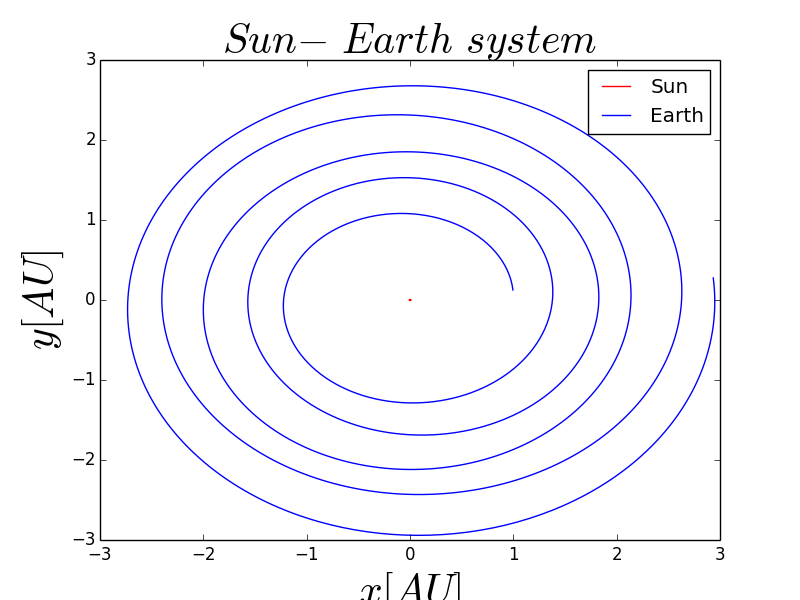
\includegraphics[width=6cm]{Euler_0_01.png}
\end{figure}
\begin{figure}[H]
\centering
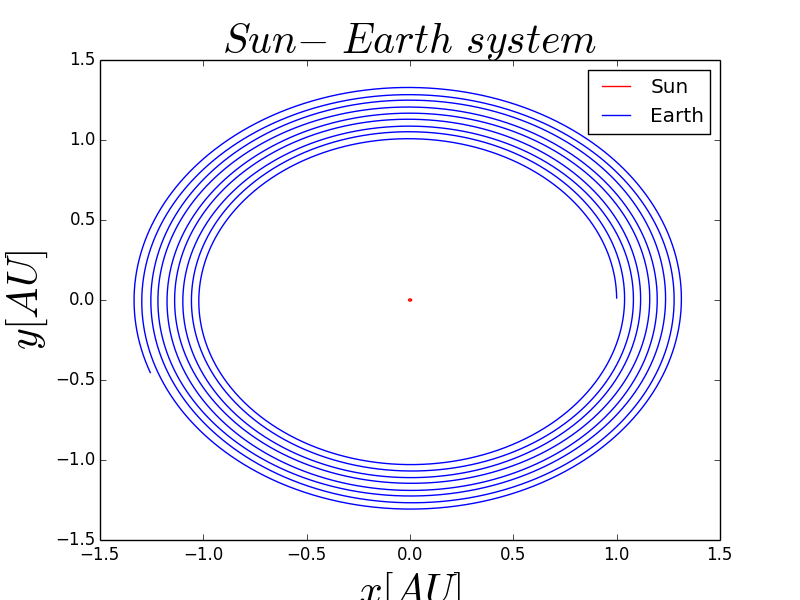
\includegraphics[width=6cm]{Euler_0_001.png}
\end{figure}
\begin{figure}[H]
\centering
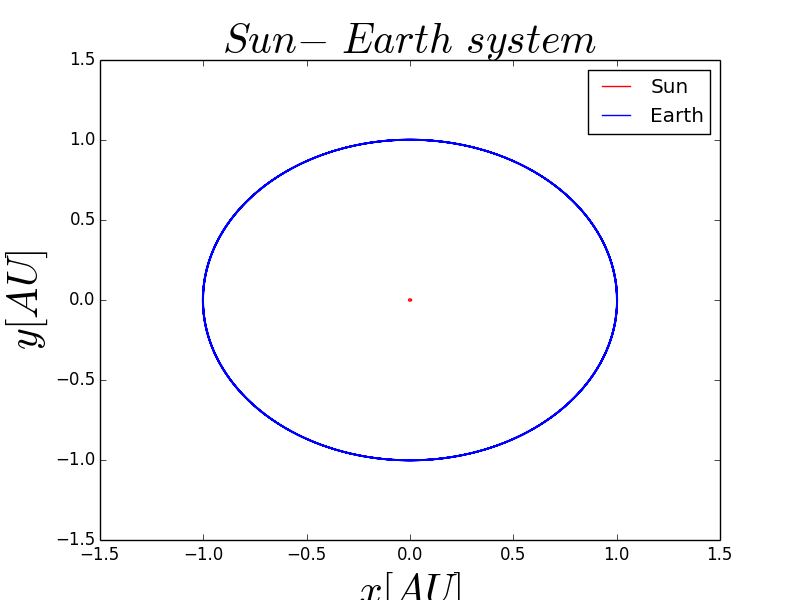
\includegraphics[width=6cm]{Euler_0_00001.png}
\caption{(Three plots in one caption) Euler method for 3 diffent dt's. Top has $dt = 0.01$, middle has $dt = 0.001$ and last $dt =0.00001$}
\end{figure}
\begin{figure}[H]
\centering
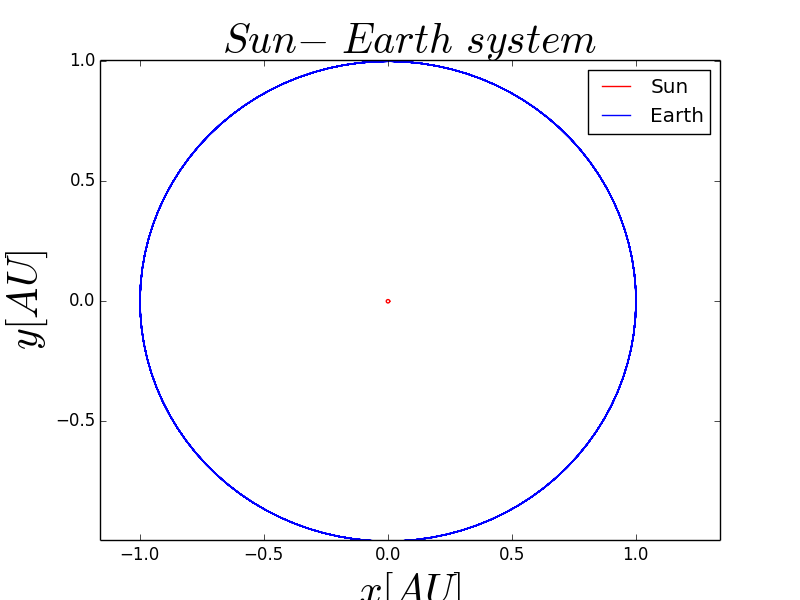
\includegraphics[width=6cm]{Verlet_0_01.png}
\end{figure}
\begin{figure}[H]
\centering
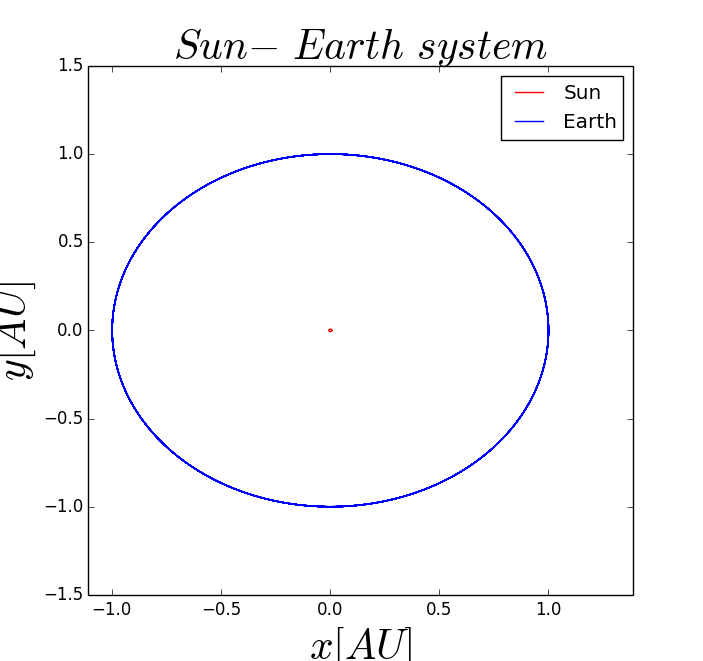
\includegraphics[width=6cm]{Verlet_0_001.png}
\end{figure}
\begin{figure}[H]
\centering
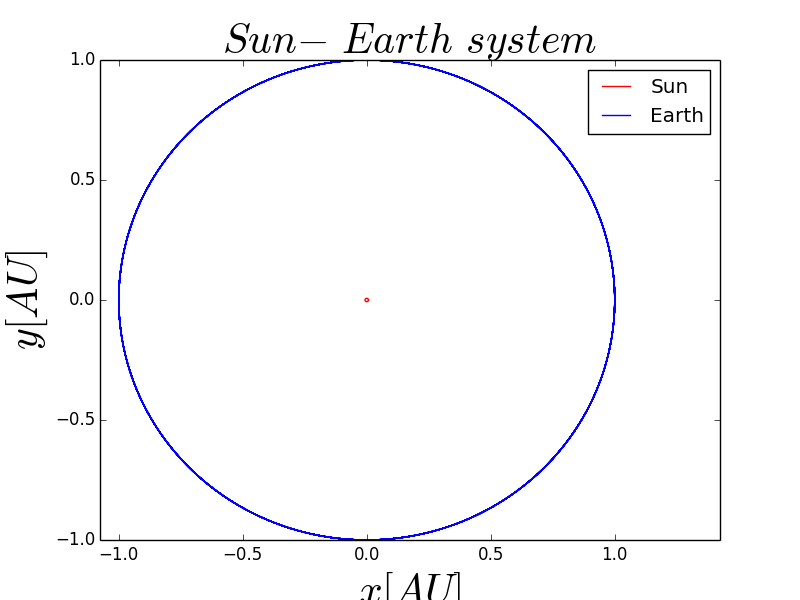
\includegraphics[width=6cm]{Verlet_0_00001.png}
\caption{(Three plots in one caption) Verlet method for 3 different dt's. Top has $dt = 0.01$, middle has $dt = 0.001$ and last $dt =0.00001$}
\end{figure}
\subsection*{Energy and angular momentum}
\begin{figure}[H]
\centering
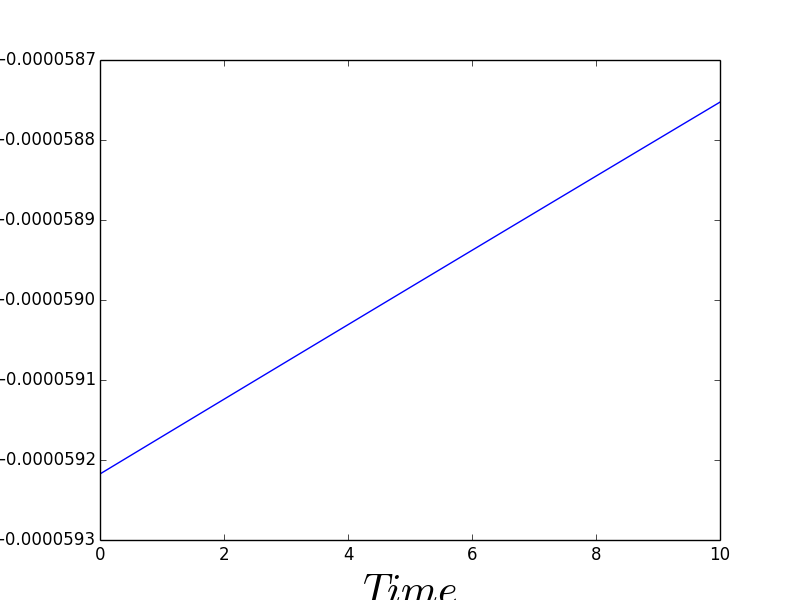
\includegraphics[width=6cm]{E_euler.png}
\end{figure}
\begin{figure}[H]
\centering
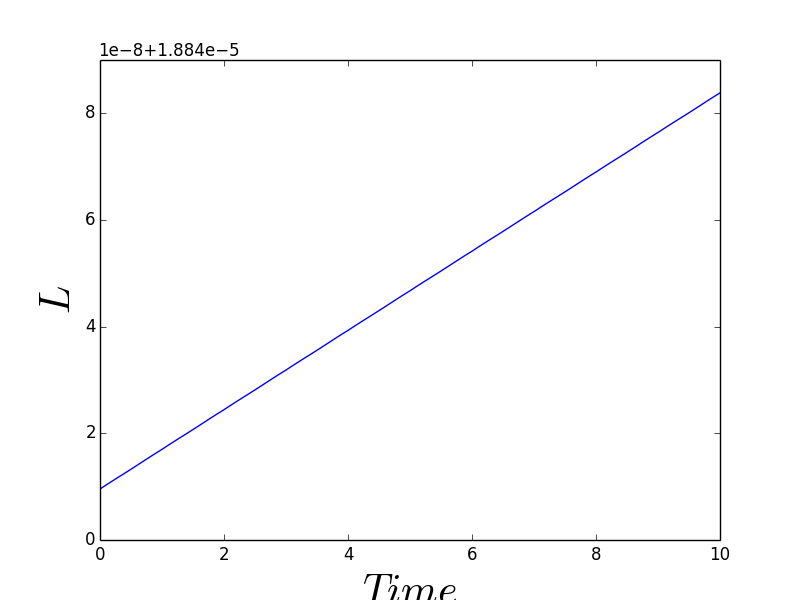
\includegraphics[width=6cm]{ang_euler.png}
\caption{(Two plots in one caption) Energy and angular momentum using the Euler method of the earth simulating of ten years. The energy plot above and angular momentum plot below.}
\end{figure}
\begin{figure}[H]
\centering
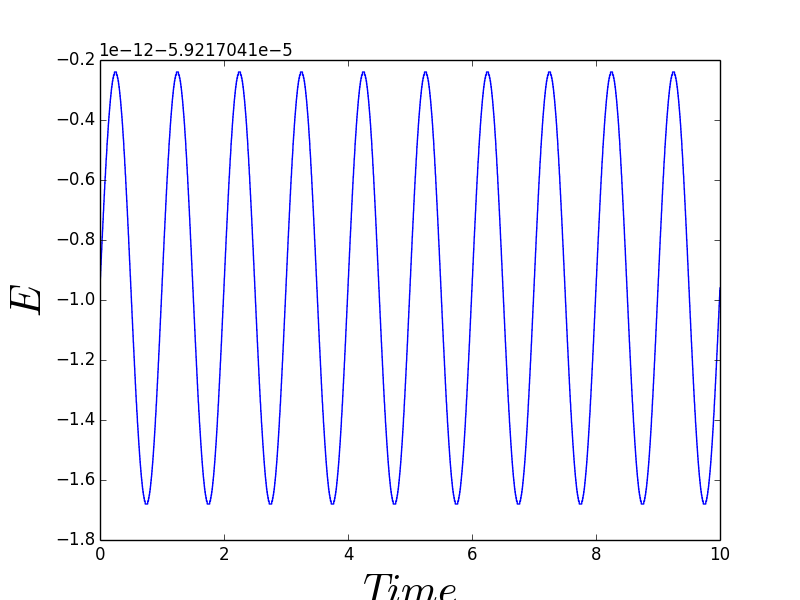
\includegraphics[width=7cm]{E_VERLET.png}
\end{figure}
\begin{figure}[H]
\centering
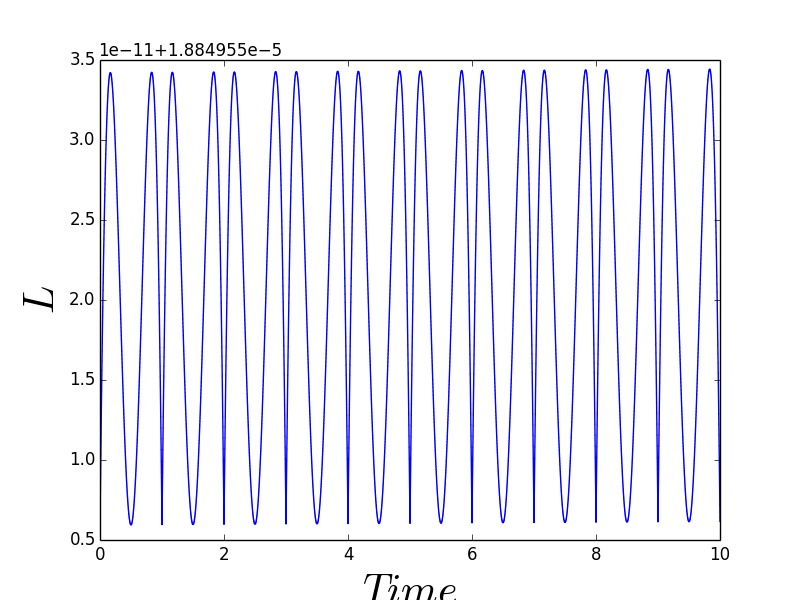
\includegraphics[width=7cm]{ang_verlet.png}
\caption{(Two plots in one caption) Energy and angular momentum using the Verlet method of the earth simulating over ten years. The energy plot above and angular momentum plot below}
\end{figure}
\begin{figure}[H]
\centering
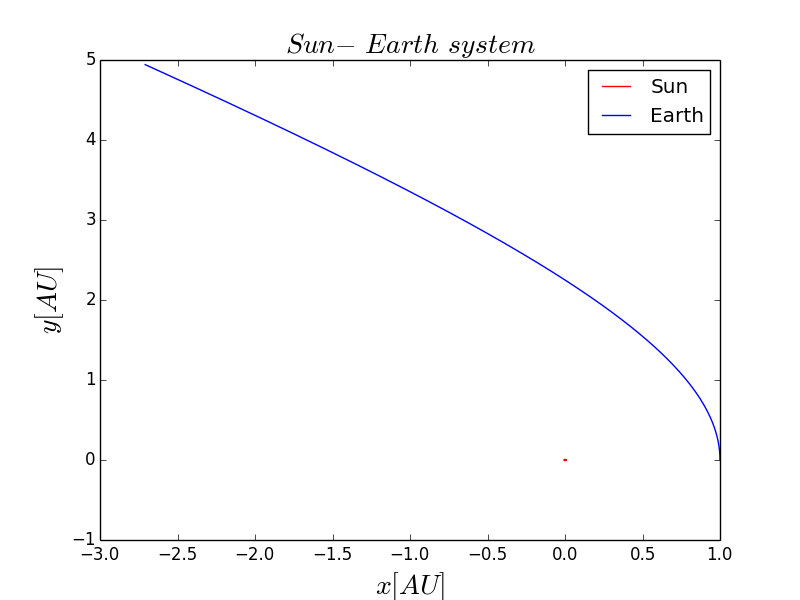
\includegraphics[width=7cm]{escvel_earth.png}
\caption{Plot of the earth sun system where the earth is given a initial velocity $3\pi$. The earth overcomes the potential energy thus moving out of orbit.}
\end{figure}
\begin{figure}[H]
\centering
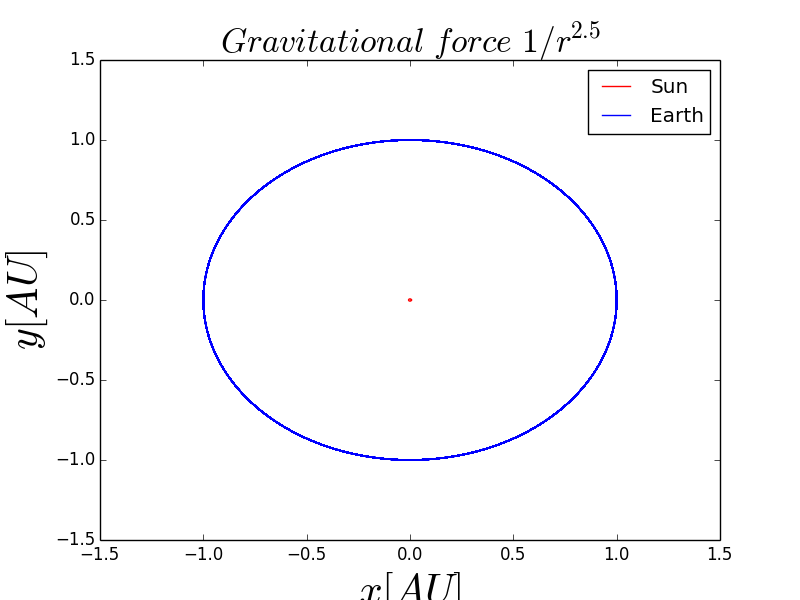
\includegraphics[width=6cm]{Gravational_force_2_5.png}
\caption{Increasing the gravitational force from $1/r^2$ to $1/r^{2.5}$ the earth's still stays in orbit.}
\end{figure}
\begin{figure}[H]
\centering
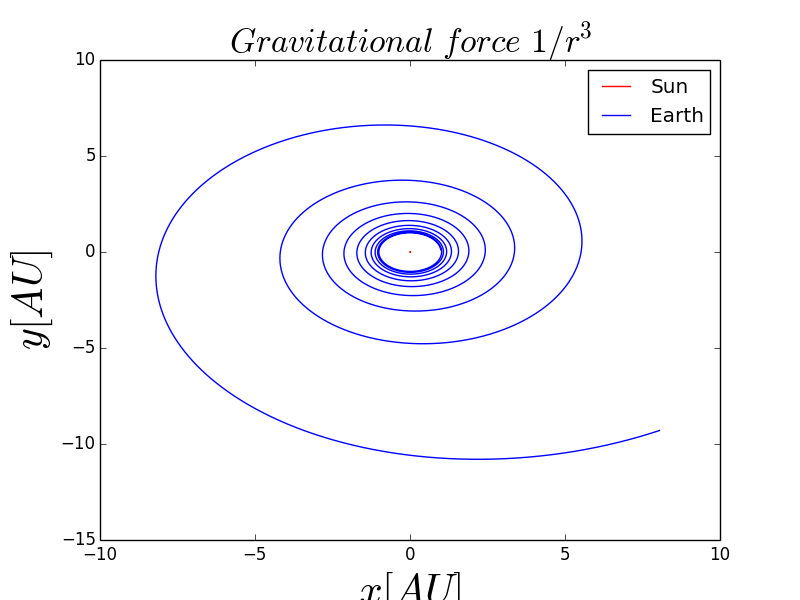
\includegraphics[width=6cm]{Gravtational_force_increase.png}
\caption{The force goes as $1/r^3$. The earth's trajectory is now clearly unstable and is slowly beginning to deviate from it's original trajectory.}
\end{figure}
\begin{figure}[H]
\centering
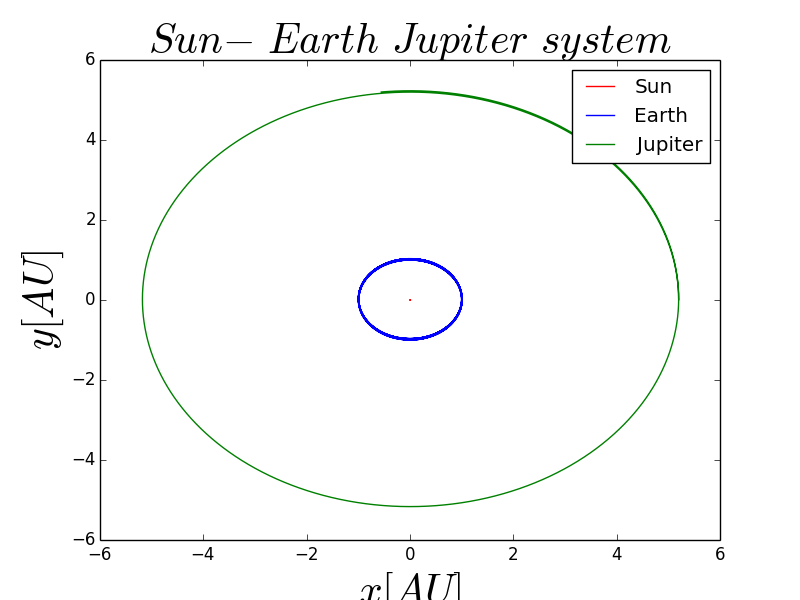
\includegraphics[width=6cm]{sun_earth_jupiter.png}
\caption{Three body problem. The Sun, Earth and Jupiter.}
\end{figure}
\begin{figure}[H]
\centering
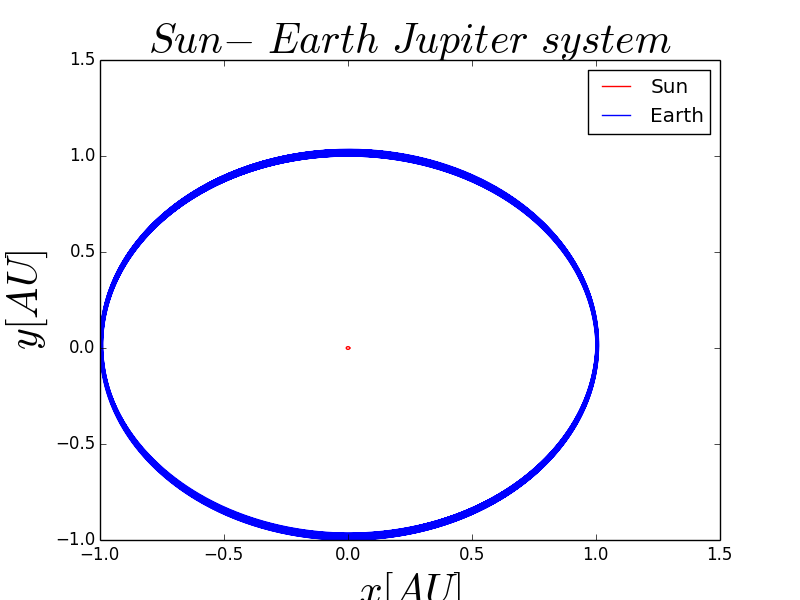
\includegraphics[width=6cm]{sun_earth_bigmass.png}
\caption{Increasing Jupiter by a factor 10. We are only interested how the earth behaves when Jupiter increases in size. The earth is getting larger and larger orbits.}
\end{figure}
\begin{figure}[H]
\centering
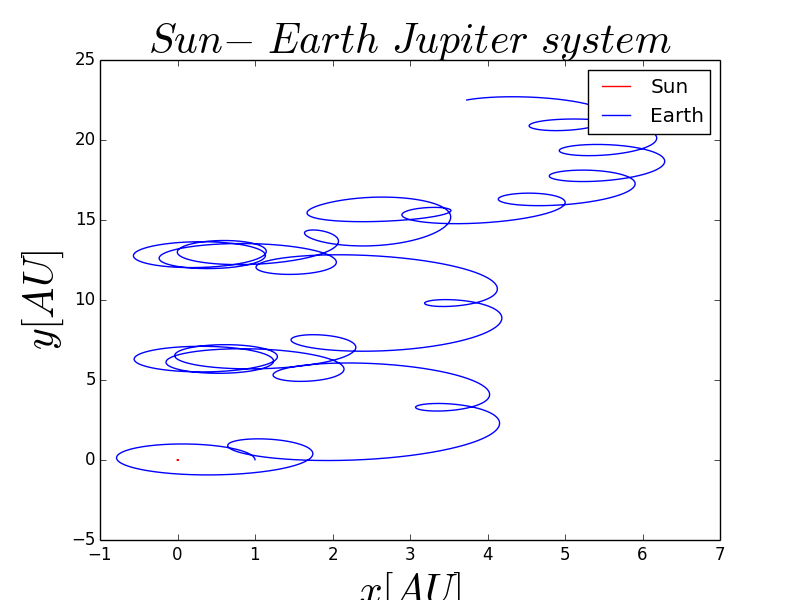
\includegraphics[width=6cm]{Sun_earth_hugemass.png}
\caption{Jupiter is now the same mass as the sun and the earth's trajectory cannot be predicted.}
\end{figure}
\begin{figure}[H]
\centering
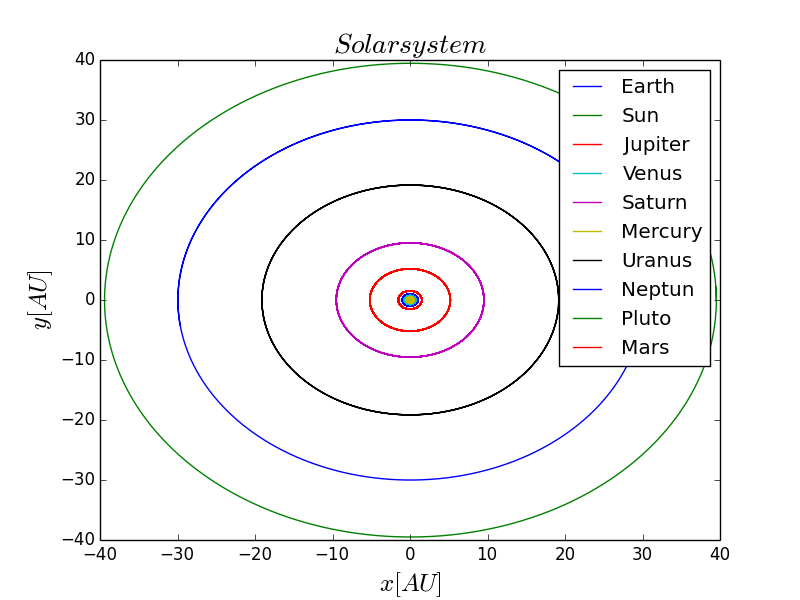
\includegraphics[width=6cm]{Solarsystem.png}
\caption{The complete solar system with pluto run over a time period of 10 years.}
\end{figure}
\begin{figure}[H]
\centering
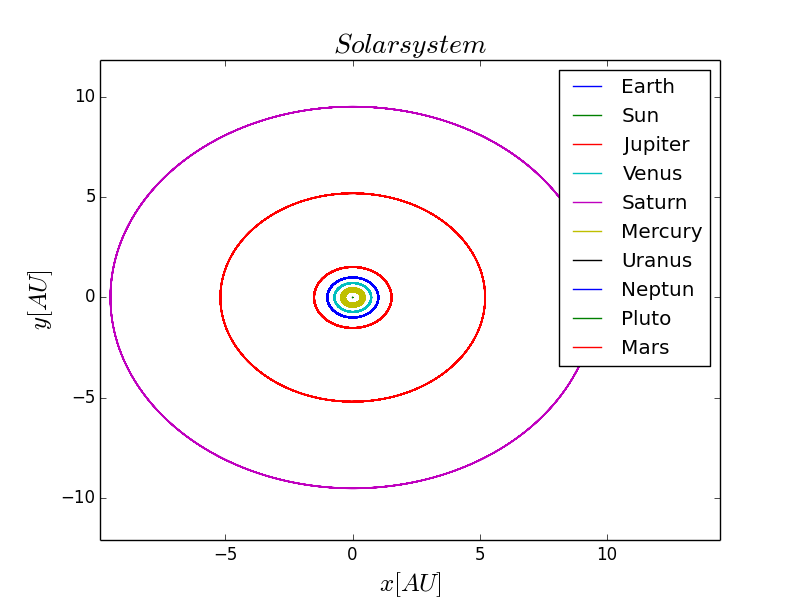
\includegraphics[width=8cm]{Solarsystem_zoom.png}
\caption{Zoomed inn plot of figure 6 showing (from biggest to smallest) Saturn, Jupiter, Earth, Mars, Venus and Mercury}
\end{figure}
\begin{figure}[H]
\centering
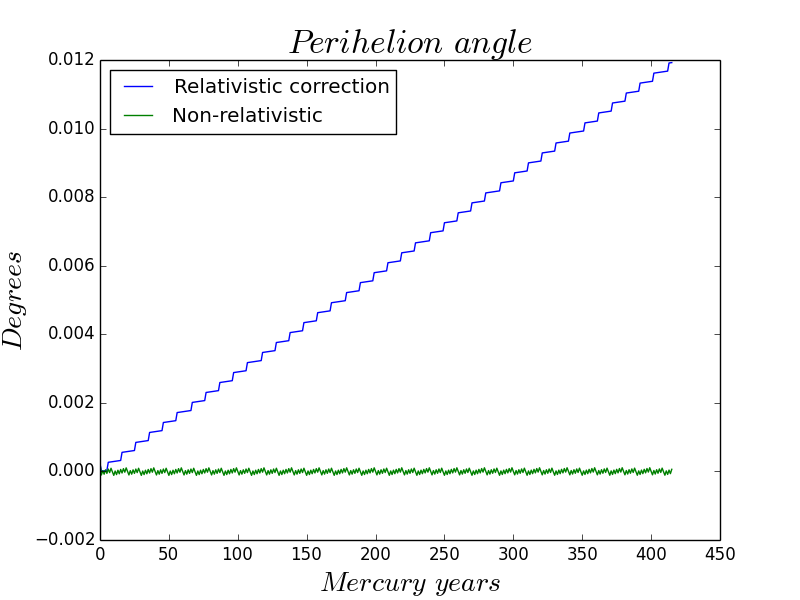
\includegraphics[width=8cm]{perihelion.png}
\caption{Mercury's perihelion angle with and without relativistic correction.}
\end{figure}
\subsection*{Link to programs}
https://github.com/Thomassjaastad/FYS-3150-Project-3/tree/master
\section*{\Romannum{4}. DISCUSSION} 
From figure 1 we see that the Euler method fails for high dt's thus making this algorithm unpractical for this use where we necessarily don't need a such fine tuned dt. A lower dt implies that we do more calculations which can be rather time consuming. The number of flops for the euler method is 5 and 6 for verlet which leads us to believe that the euler method should be a more efficient algorithm, but from the latter this is not the case because the choice of dt also as an effect on the run- time of the algorithms. The Euler method has an error that goes as $NO(dt^2) \approx O(dt)$ where $N = (t_n - t_0)/dt$. It is clear from figure 2 that Verlet does not suffer from this change in dt which has an error that goes as $O(dt^3)$. We also see from figure 3 and 4 that the verlet algorithm conserves the energy where the euler method does not. We expect that the energy and angular momentum are conserved when no external forces are acting on the object. The reason for the oscillating energy and angular momentum is because of the circular motion of the planet which is assumed in this project. Both the energy and momentum depend on the position of the object, so when the position changes, the energy and momentum does also.  

The escape velocity can derived from the total energy $E_{tot} = E_k + E_p$ where $E_k = 0.5mv^2$ and $E_p = -GMm/r$. Solving for the velocity v we find $v > \sqrt{2Gm/r}$ the boundary for the escape velocity. (see figure 5 for escape velocity plot). If we increase the power of the radial distance the velocity needed to escape the suns gravitational potential is lower than if the power is $r^2$. Increasing the power by one we get $E_p = -GMm/r^2$, this leads to $v > \sqrt{2Gm/r^2}$. In figure 6 and 7 we see that the earth- sun system the gravitational force is not stable when increasing the force from $1/r^2$ to $1/r^3$.    

Making Jupiter as large as the sun made the earth's trajectory none circular, because now two objects are pulling at the earth with almost the same force, besides the distance between the objects. The Verlet algorithm is still capable of calculating the earths trajectory.  

After adding all planets inn the solar system, Pluto included, the motions look reasonable where the expected orbit is circular (see figure 9 and 10). It does not look as though the center of mass correction had much effect on the whole system. The sun has a mass with magnitude of 3 larger than the next largest planet in the solar system, so it is not necessarily so odd that the center of mass contributes little comparing with the sun fixed in origo.

Mercury's orbit after one century(which equals 415 mercury years) we find that the angle at perihelion is $0.011924 \degree$ which is what we expect from observed values. It is of importance to include enough time steps where this accounts to how precis the calculation of the angle is or else we will not possibly include the lowest point in the orbit. Another importance was to show that theory of general relativity predicted this perihelion precession which it did. See figure 13 for plot. 
\section*{\Romannum{5}. CONCLUSION}
The verlet algorithm produced better results than the euler method, being able to do many calculations with a higher precision than euler, where euler suffered from error's becoming large when looking at the system for a large time period. The verlet algorithm was also capable of calculating the earth's trajectory when the mass of jupiter increased.

It was good to check the energy and angular momentum too see if these quantities were conserved, which they were. One odd notification was that the energy and angular momentum didn't always seem to be conserved for all chosen dt's (for lower values of dt), the reason for this is unknown. One possibility could be that the change in energy and angular momentum is too small that the computer suffers from numerical precision. 

Calculating mercury's perihelion gave a satisfactory result compared to Einstein's theory of relativity where the analytic value is $43'' = 0.011943 \degree$ and our numerical value was found to be $\theta_p = 0.011924\degree$.
\newpage
\section*{\Romannum{6}. REFERENCES}
Hjort -Jensen Morten., 2015. Computational Physics Kompendiet. 
\newline
http://compphysics.github.io/ComputationalPhysics/doc/pub/linalg/pdf/linalg-print.pdf 
\end{document}
